\documentclass{beamer}
% Use DS9 global theme (includes pgfplots for visualization)
\usepackage{../../../../latex-beamer/shared/templates/ds9_theme}

% Title page configuration
\title[Newton's Laws and Systems]{PHYS12 CH: 4.1-4.4, 4.6-4.8}
\subtitle{Force, Mass, Systems, and Fundamental Forces}
\author[Mr. Gullo]{Mr. Gullo}
\date[Sep 2024]{September 17, 2024}

\begin{document}
\frame{\titlepage}

\section{Introduction}

\begin{frame}
\frametitle{Learning Objectives}
\begin{itemize}
    \item Understand the definition of \textbf{force} as a vector. \pause
    \item Define \textbf{mass} and \textbf{inertia}. \pause
    \item State and apply Newton's First, Second, and Third Laws of Motion. \pause
    \item Define a \textbf{system of interest} and distinguish between \textbf{external} and \textbf{internal} forces. \pause
    \item Draw and use \textbf{Free-Body Diagrams (FBDs)} to solve problems. \pause
    \item Apply Newton's laws to solve problems for both single objects and multi-body systems. \pause
    \item Analyze complex two-dimensional force problems with vector addition. \pause
    \item Identify and describe the \textbf{four fundamental forces} of nature and their properties. \pause
    \item Understand how forces act at a distance through \textbf{force fields} and particle exchange.
\end{itemize}
\end{frame}

\begin{frame}
\frametitle{From Physics 11 to Physics 12}
\begin{columns}[T]
\column{0.48\textwidth}
\begin{alertblock}{Review from Physics 11}
\begin{itemize}
    \item Newton's Laws for a \textbf{single object}.
    \item Drawing a Free-Body Diagram for one object.
    \item Identifying forces like gravity ($\vec{w}$), normal force ($\vec{N}$), and tension ($\vec{T}$).
    \item Solving for acceleration or force on one object using $\sum \vec{F} = m\vec{a}$.
\end{itemize}
\end{alertblock}

\column{0.48\textwidth}
\begin{exampleblock}{New in Physics 12}
\begin{itemize}
    \item Applying Newton's Laws to \textbf{systems of multiple objects}.
    \item Strategically choosing the "system of interest" to simplify problems.
    \item Understanding how internal forces cancel out within a system.
    \item Solving for forces between connected objects.
\end{itemize}
\end{exampleblock}
\end{columns}
\end{frame}

\section{Fundamental Concepts Review}

\begin{frame}
\frametitle{Concept: What is a Force?}
\begin{itemize}
    \item A force is fundamentally a \textbf{push} or a \textbf{pull}. \pause
    \item It is a \textbf{vector quantity}, meaning it has both \alert{magnitude} (how strong it is) and \alert{direction}. \pause
    \item The standard unit of force is the \textbf{Newton (N)}.
    \begin{itemize}
        \item 1 N = 1 kg $\cdot$ m/s$^2$
    \end{itemize} \pause
    \item Forces are added together using vector addition to find the \textbf{net force} ($\vec{F}_{net}$).
\end{itemize}
\end{frame}

\begin{frame}
\frametitle{Concept: The Free-Body Diagram (FBD)}
A Free-Body Diagram is a simplified drawing used to analyze the forces on an object or system.
\begin{itemize}
    \item The system of interest is represented by a single \textbf{dot}. \pause
    \item We draw vector arrows representing all \textbf{external forces} acting \textit{on} the system. \pause
    \item We do \textbf{not} draw internal forces or forces exerted \textit{by} the system. \pause
    \item The FBD is the most critical first step for solving almost any dynamics problem.
\end{itemize}
\end{frame}

\begin{frame}
\frametitle{Context: Visualizing Net Force}
\begin{itemize}
    \item Let's visualize how forces on an object combine to produce a net force using a Free-Body Diagram.
    \pause
    \item We will use the example of two ice skaters pushing a third skater from Figure 4.3 in your textbook.
    \pause
    \item The two pushes ($\vec{F}_1$ and $\vec{F}_2$) are individual external forces. The \textbf{net force} ($\vec{F}_{tot}$) is their vector sum, which determines the direction of acceleration.
\end{itemize}
\end{frame}

\begin{frame}
\frametitle{Visualization: Adding Forces on an FBD}
\begin{alertblock}{[Diagram based on Figure 4.3]}
\begin{columns}[T]
\column{0.5\textwidth}
    \textbf{Physical Situation:}
    \begin{itemize}
        \item An overhead view shows two skaters applying forces $\vec{F}_1$ and $\vec{F}_2$ to a third skater.
    \end{itemize}
    \alert{[Image of two skaters pushing a third skater]}
\column{0.5\textwidth}
    \textbf{Free-Body Diagram:}
    \begin{itemize}
        \item The third skater is a dot.
        \item $\vec{F}_1$ and $\vec{F}_2$ are drawn tail-to-dot.
        \item The resultant vector $\vec{F}_{tot}$ shows the net force.
    \end{itemize}
    \alert{[FBD showing two force vectors from a point]}
\end{columns}
\end{alertblock}
\end{frame}

\begin{frame}
\frametitle{Newton's First Law: The Law of Inertia}
\begin{itemize}
    \item "A body at rest remains at rest, or, if in motion, remains in motion at a constant velocity unless acted on by a \textbf{net external force}." \pause
    \item This means an object's velocity \textbf{will not change} if the net force on it is zero ($\vec{F}_{net} = 0$). \pause
    \item \textbf{Inertia} is the property of an object to resist changes in its state of motion. \pause
    \item \textbf{Mass (m)} is the quantitative measure of inertia. More mass means more inertia.
\end{itemize}
\end{frame}

\begin{frame}
\frametitle{Newton's Third Law: Action-Reaction}
\begin{itemize}
    \item "Whenever one body exerts a force on a second body, the first body experiences a force that is equal in magnitude and opposite in direction to the force that it exerts." \pause
    \item Mathematically: $\vec{F}_{A \text{ on } B} = -\vec{F}_{B \text{ on } A}$ \pause
    \item \alert{CRITICAL POINT}: The two forces in an action-reaction pair always act on \textbf{different objects}. \pause
    \begin{itemize}
        \item Therefore, they \textbf{never} cancel each other out when analyzing the motion of a single object.
    \end{itemize}
\end{itemize}
\end{frame}

\begin{frame}
\frametitle{Context: Visualizing Action-Reaction}
\begin{itemize}
    \item Let's visualize how action-reaction pairs work. The key is to see that the forces act on different systems. \pause
    \item We will look at a swimmer pushing off the wall of a pool (based on Figure 4.9). \pause
    \item The "action" is the swimmer pushing on the wall.
    \item The "reaction" is the wall pushing on the swimmer. Only the reaction force affects the swimmer's motion.
\end{itemize}
\end{frame}

\begin{frame}
\frametitle{Visualization: Swimmer at the Wall}
\begin{alertblock}{[Diagram based on Figure 4.9]}
    \begin{itemize}
        \item \textbf{Force 1 (Action):} The swimmer's feet exert a force $\vec{F}_{feet\_on\_wall}$ on the wall. This force acts ON THE WALL.
        \pause
        \item \textbf{Force 2 (Reaction):} The wall exerts an equal and opposite force $\vec{F}_{wall\_on\_feet}$ on the swimmer. This force acts ON THE SWIMMER.
        \pause
        \item The swimmer accelerates because the net external force on \textit{her} (from the wall) is not zero.
    \end{itemize}
    \alert{[Image showing swimmer pushing off a wall, with force vectors on both swimmer and wall]}
\end{alertblock}
\end{frame}

\section{The Concept of a System}

\begin{frame}
\frametitle{The "System": A Key Problem-Solving Tool}
\begin{itemize}
    \item In physics, a \textbf{system} is the object or collection of objects we choose to analyze. \pause
    \item \textbf{External forces} act on the system from the outside.
    \begin{itemize}
        \item These are the forces that cause the system to accelerate.
        \item They are the only forces shown on an FBD of the system.
    \end{itemize} \pause
    \item \textbf{Internal forces} are forces that objects within the system exert on each other.
    \begin{itemize}
        \item These forces always come in action-reaction pairs and cancel out, so they \textbf{do not affect the system's overall acceleration}.
    \end{itemize}
\end{itemize}
\end{frame}

\begin{frame}
\frametitle{Context: Choosing a System}
\begin{itemize}
    \item The choice of system is a strategic decision that can make a problem much easier to solve. \pause
    \item Let's see how changing the system changes which forces are external. \pause
    \item We'll use the example of a professor pushing a cart from Figure 4.10.
\end{itemize}
\end{frame}

\begin{frame}
\frametitle{Visualization: Professor and Cart Systems}
\begin{alertblock}{[Diagram based on Figure 4.10]}
\begin{columns}[T]
\column{0.48\textwidth}
    \textbf{System 1: (Professor + Cart)}
    \begin{itemize}
        \item External forces: Force from floor on feet, friction.
        \item Internal force: Professor pushing cart, cart pushing professor. These cancel.
    \end{itemize}
\column{0.48\textwidth}
    \textbf{System 2: (Cart Only)}
    \begin{itemize}
        \item External forces: Force from professor on cart, friction.
        \item No internal forces to consider.
    \end{itemize}
\end{columns}
\alert{[Image showing a professor pushing a cart, with boxes drawn around "System 1" and "System 2"]}
\end{alertblock}
\end{frame}

\begin{frame}
\frametitle{Newton's Second Law: The Law of Acceleration}
\begin{itemize}
    \item "The acceleration of a system is directly proportional to and in the same direction as the \textbf{net external force} acting on the system, and is inversely proportional to its total mass." \pause
    \item This is the central, quantitative law of dynamics. It connects force, mass, and motion.
\end{itemize}
\end{frame}

\begin{frame}
\frametitle{Essential Equations}
\begin{block}{Newton's Second Law}
\centering
$\vec{F}_{net} = m\vec{a}$
\begin{itemize}
    \item $\vec{F}_{net}$ is the vector sum of all \textit{external} forces on the system.
    \item $m$ is the total mass of the system.
    \item $\vec{a}$ is the acceleration of the system.
\end{itemize}
\end{block}
\pause
\begin{block}{Weight (Force of Gravity)}
\centering
$\vec{w} = m\vec{g}$
\begin{itemize}
    \item $\vec{w}$ is the force of gravity on an object.
    \item $m$ is the object's mass.
    \item $\vec{g}$ is the acceleration due to gravity (approx. 9.8 m/s$^2$ down on Earth).
\end{itemize}
\end{block}
\end{frame}

\section{Problem Solving with Systems}

\begin{frame}
\frametitle{I Do: Getting up to Speed (Example 4.3)}
\begin{block}{Problem}
A professor (65.0 kg) pushes a cart (12.0 kg) with equipment (7.0 kg). She exerts a 150 N backward force on the floor. All forces opposing the motion total 24.0 N. Calculate the acceleration.
\end{block}
\pause
\begin{alertblock}{System of Interest}
For this question, our system is the \textbf{professor + cart + equipment} because we want the acceleration of everything together.
\end{alertblock}
\end{frame}

\begin{frame}
\frametitle{I Do: GUESS Method (G \& U)}
\begin{columns}[T]
\column{0.48\textwidth}
\textbf{G - Givens}
\begin{itemize}
\item $m_{prof} = 65.0$ kg
\item $m_{cart} = 12.0$ kg
\item $m_{equip} = 7.0$ kg
\item Force on floor = 150 N
\item $\implies F_{floor\_on\_prof} = 150$ N [forward]
\item $f = 24.0$ N [backward]
\end{itemize}

\column{0.48\textwidth}
\textbf{U - Unknown}
\begin{itemize}
\item Acceleration, $a = ?$
\end{itemize}
\end{columns}
\end{frame}

\begin{frame}
\frametitle{I Do: GUESS Method (E)}
\textbf{E - Equation}
\begin{itemize}
    \item Start with Newton's Second Law for the whole system:
    \[ F_{net} = m_{total} a \] \pause
    \item The net external force is the forward force from the floor minus the backward friction:
    \[ F_{net} = F_{floor\_on\_prof} - f \] \pause
    \item The total mass is the sum of all parts:
    \[ m_{total} = m_{prof} + m_{cart} + m_{equip} \] \pause
    \item Rearrange for the unknown, $a$:
    \[ a = \frac{F_{net}}{m_{total}} = \frac{F_{floor\_on\_prof} - f}{m_{prof} + m_{cart} + m_{equip}} \]
\end{itemize}
\end{frame}

\begin{frame}
\frametitle{I Do: GUESS Method (S \& S)}
\textbf{S - Substitute}
\begin{itemize}
    \item First, calculate total mass:
    \[ m_{total} = 65.0 + 12.0 + 7.0 = 84.0 \text{ kg} \]
    \item Now substitute into the acceleration equation:
    \[ a = \frac{150 \text{ N} - 24.0 \text{ N}}{84.0 \text{ kg}} \]
\end{itemize}
\pause
\textbf{S - Solve}
\begin{itemize}
    \item Calculate the final value:
    \[ a = \frac{126 \text{ N}}{84.0 \text{ kg}} = 1.5 \text{ m/s}^2 \]
    \item \boxed{a = 1.5 \text{ m/s}^2 \text{ [forward]}}
\end{itemize}
\end{frame}

\begin{frame}
\frametitle{We Do: Force on the Cart (Example 4.4)}
\begin{block}{Problem}
Using the data from the previous problem, calculate the force the professor exerts on the cart.
\end{block}
\pause
\begin{alertblock}{New System of Interest}
Now, our system must be the \textbf{cart + equipment} because the force from the professor is an \textit{external force} on this new system.
\end{alertblock}
\end{frame}

\begin{frame}
\frametitle{We Do: GUESS Method (G \& U)}
\begin{columns}[T]
\column{0.48\textwidth}
\textbf{G - Givens}
\begin{itemize}
\item $m_{cart} = 12.0$ kg
\item $m_{equip} = 7.0$ kg
\item $m_{sys2} = 19.0$ kg
\item $a = 1.5$ m/s$^2$ (from "I do")
\item $f_{total} = 24.0$ N (The problem states this friction applies to cart wheels and air resistance, so it acts on the cart system).
\end{itemize}

\column{0.48\textwidth}
\textbf{U - Unknown}
\begin{itemize}
\item Force from professor on cart, $F_{prof} = ?$
\end{itemize}
\end{columns}
\end{frame}

\begin{frame}
\frametitle{We Do: GUESS Method (E)}
\textbf{E - Equation}
\begin{itemize}
    \item Apply Newton's Second Law to our new system (the cart + equipment):
    \[ F_{net} = m_{sys2} a \]
    \pause
    \item \textbf{Question:} What forces make up $F_{net}$ for this system?
    \begin{itemize}
        \item \textit{Answer: The forward push from the professor ($F_{prof}$) and the backward friction ($f$).}
        \[ F_{prof} - f = m_{sys2} a \]
    \end{itemize}
    \pause
    \item \textbf{Question:} How do we rearrange for the unknown, $F_{prof}$?
    \begin{itemize}
        \item \textit{Answer: Add friction $f$ to both sides.}
        \[ F_{prof} = m_{sys2} a + f \]
    \end{itemize}
\end{itemize}
\end{frame}

\begin{frame}
\frametitle{We Do: GUESS Method (S \& S)}
\textbf{S - Substitute}
\begin{itemize}
    \item Now we plug in the values for our system.
    \pause
    \item \textbf{Question:} What values should we use for $m_{sys2}$, $a$, and $f$?
    \begin{itemize}
        \item $m_{sys2} = 19.0$ kg
        \item $a = 1.5$ m/s$^2$
        \item $f = 24.0$ N
    \end{itemize}
    \[ F_{prof} = (19.0 \text{ kg})(1.5 \text{ m/s}^2) + 24.0 \text{ N} \]
\end{itemize}
\pause
\textbf{S - Solve}
\begin{itemize}
    \item Let's calculate the result.
    \[ F_{prof} = 28.5 \text{ N} + 24.0 \text{ N} = 52.5 \text{ N} \]
    \item \boxed{F_{prof} = 53 \text{ N}}
\end{itemize}
\end{frame}

\begin{frame}
\frametitle{You Do: Drag Force on a Barge (Example 4.7)}
\begin{block}{Problem}
Two tugboats push on a barge. Tugboat 1 exerts a force of $2.7 \times 10^5$ N in the x-direction. Tugboat 2 exerts a force of $3.6 \times 10^5$ N in the y-direction. The mass of the barge is $5.0 \times 10^6$ kg and its acceleration is observed to be $7.5 \times 10^{-2}$ m/s$^2$ in the direction of the net applied force from the tugboats.
\newline
\newline
What is the drag force of the water on the barge resisting the motion?
\end{block}

\begin{alertblock}{Hint}
1. Find the magnitude and direction of the total applied force from the tugboats.
2. Calculate the net force needed to cause the observed acceleration ($F_{net}=ma$).
3. The drag force is the difference between the applied force and the net force.
\end{alertblock}
\end{frame}

\section{Additional Worked Examples}

\begin{frame}
\frametitle{Example: Rugby Players (Problem 16)}
A rugby player (90.0 kg) is accelerating at $1.20 \mathrm{~m} / \mathrm{s}^{2}$ backward while being pushed by an opposing player exerting 800 N.
\begin{itemize}
    \item[(a)] What is the force of friction between the losing player's feet and the grass?
    \item[(b)] What force must the winning player (110 kg) exert on the ground to move forward at the same acceleration?
\end{itemize}
\end{frame}

\begin{frame}
\frametitle{Problem 16 - Solution (a)}
\begin{columns}[T]
    \column{0.5\textwidth}
        \begin{block}{System of Interest: Losing Player}
            \begin{itemize}
                \item $F_{\text{net}} = F_{push} - f = ma$
                \item $f = F_{push} - ma$
                \item $f = 800 \text{ N} - (90.0 \text{ kg})(1.20 \text{ m/s}^2)$
                \item $f = 800 \text{ N} - 108 \text{ N}$
                \item \boxed{f = 692 \text{ N}}
            \end{itemize}
        \end{block}
    \column{0.5\textwidth}
        \begin{figure}
            \centering
            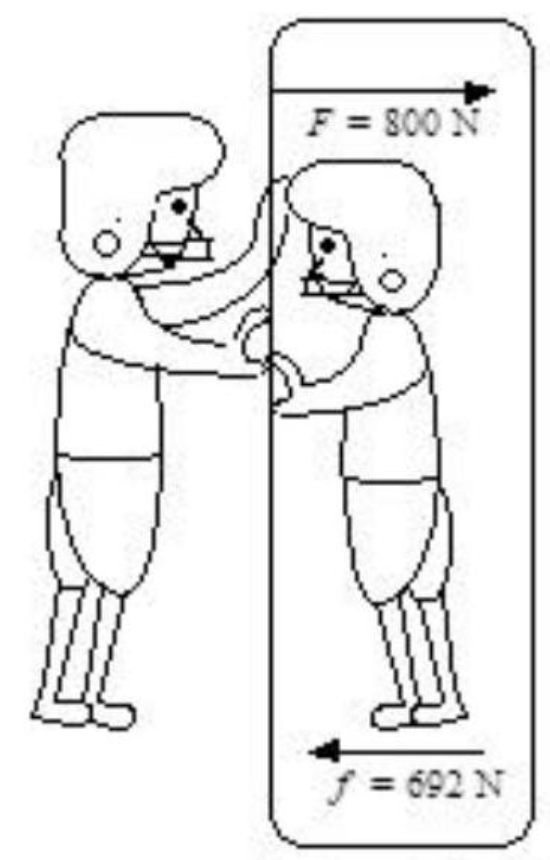
\includegraphics[width=0.7\linewidth]{Screenshot 2024-10-18 111640.png}
        \end{figure}
\end{columns}
\end{frame}

\begin{frame}
\frametitle{Problem 16 - Solution (b)}
\begin{columns}[T]
    \column{0.5\textwidth}
        \begin{block}{System of Interest: Both Players}
            \begin{itemize}
                \item Let $F_{ground}$ be the force the winner exerts on the ground.
                \item $F_{net} = F_{ground} - f = (m_1+m_2)a$
                \item $F_{ground} = (m_1+m_2)a + f$
                \item $F_{ground} = (90.0+110)\text{kg}(1.20 \text{m/s}^2) + 692 \text{N}$
                \item $F_{ground} = 240 \text{N} + 692 \text{N}$
                \item \boxed{F_{ground} = 932 \text{N}}
            \end{itemize}
        \end{block}
    \column{0.5\textwidth}
        \begin{figure}
            \centering
            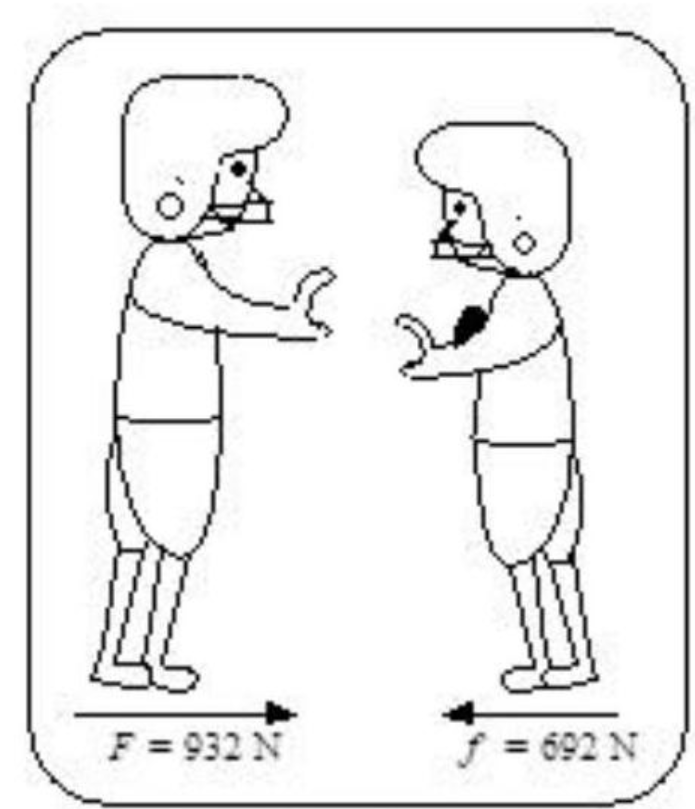
\includegraphics[width=0.7\linewidth]{Screenshot 2024-10-18 111809.png}
        \end{figure}
\end{columns}
\end{frame}

\section{Conclusion}

\section{Section 4.7: Further Applications}

\begin{frame}
\frametitle{Section 4.7: Further Applications of Newton's Laws}
\framesubtitle{Complex Systems and Multi-Dimensional Forces}
\begin{itemize}
    \item Newton's laws apply to more complex scenarios: \pause
    \begin{itemize}
        \item Two-dimensional force problems with vector addition
        \item Objects with multiple forces at different angles
        \item Real-world applications with drag and resistance
    \end{itemize} \pause
    \item These problems integrate kinematics with dynamics \pause
    \item Strategic use of coordinate systems and trigonometry is essential
\end{itemize}
\end{frame}

\begin{frame}
\frametitle{Example: Drag Force on a Barge (Example 4.7)}
\begin{block}{Problem Summary}
Two tugboats push a barge at perpendicular angles ($F_1 = 2.7 \times 10^5$ N in x-direction, $F_2 = 3.6 \times 10^5$ N in y-direction). The barge (mass $5.0 \times 10^6$ kg) accelerates at $7.5 \times 10^{-2}$ m/s$^2$. Find the drag force.
\end{block}
\pause
\begin{alertblock}{Solution Approach}
\begin{itemize}
    \item Find total applied force: $F_{app} = \sqrt{F_1^2 + F_2^2} = 4.5 \times 10^5$ N
    \item Apply Newton's 2nd Law: $F_{net} = F_{app} - F_D = ma$
    \item Result: $F_D = 7.5 \times 10^4$ N (opposite to motion direction)
\end{itemize}
\end{alertblock}
\end{frame}

\begin{frame}
\frametitle{Visualization: Barge Problem (Figure 4.21)}
\begin{alertblock}{[Diagram based on Figure 4.21]}
\textbf{Two-Dimensional Force Analysis:}
\begin{itemize}
    \item Two tugboats apply perpendicular forces to a barge
    \item Force vectors add using Pythagorean theorem
    \item Resultant $\vec{F}_{app}$ points at angle: $\theta = \tan^{-1}(F_2/F_1) = 53°$
    \item Drag force $\vec{F}_D$ opposes motion (fluid resistance)
    \item Net force determines acceleration via $\vec{F}_{net} = m\vec{a}$
\end{itemize}
\alert{[Image: Top view of barge with two tugboat force vectors and drag]}
\end{alertblock}
\end{frame}

\section{Section 4.8: Four Basic Forces}

\begin{frame}
\frametitle{Section 4.8: The Four Basic Forces}
\framesubtitle{Understanding the Fundamental Forces of Nature}
\begin{itemize}
    \item One of the most remarkable simplifications in physics: \pause
    \item \alert{Only four distinct forces account for ALL known phenomena} \pause
    \item Nearly all forces we experience directly are due to ONE basic force: the electromagnetic force \pause
    \item The gravitational force is the only other force we experience directly
\end{itemize}
\end{frame}

\begin{frame}
\frametitle{The Four Basic Forces}
\begin{enumerate}
    \item \textbf{Gravitational Force} \pause
    \item \textbf{Electromagnetic Force} \pause
    \item \textbf{Weak Nuclear Force} \pause
    \item \textbf{Strong Nuclear Force}
\end{enumerate}
\pause
\vspace{1em}
\begin{alertblock}{Key Concept}
All forces act through the exchange of microscopic carrier particles. The characteristics of basic forces are determined by the types of particles exchanged.
\end{alertblock}
\end{frame}

\begin{frame}
\frametitle{Properties of the Four Basic Forces}
\begin{table}
\scriptsize
\begin{tabular}{|l|c|c|c|c|}
\hline
\textbf{Force} & \textbf{Strength} & \textbf{Range} & \textbf{Type} & \textbf{Carrier} \\
\hline
Gravitational & $10^{-38}$ & $\infty$ & Attractive only & Graviton \\
\hline
Electromagnetic & $10^{-2}$ & $\infty$ & Both & Photon \\
\hline
Weak Nuclear & $10^{-6}$ & $< 10^{-18}$ m & Both & $W^+, W^-, Z^0$ \\
\hline
Strong Nuclear & $1$ & $\approx 10^{-15}$ m & Both & Gluons \\
\hline
\end{tabular}
\end{table}
\pause
\vspace{0.5em}
\begin{itemize}
    \item Strengths are \textbf{relative} to the strong nuclear force
    \item Nuclear forces act over extremely short ranges (size of nucleus or less)
\end{itemize}
\end{frame}

\begin{frame}
\frametitle{Gravitational Force}
\begin{itemize}
    \item \textbf{Weakest} of all forces (relative strength: $10^{-38}$) \pause
    \item Always \textbf{attractive} — this is why we notice it despite its weakness \pause
    \item \textbf{Long-range}: acts over infinite distances \pause
    \item Dominant force on astronomical scales (planets, stars, galaxies) \pause
    \item Affects the nature of space and time (general relativity) \pause
    \item \textbf{Carrier particle}: Graviton (proposed but not yet observed)
\end{itemize}
\end{frame}

\begin{frame}
\frametitle{Electromagnetic Force}
\begin{itemize}
    \item Combination of electrical forces and magnetic forces \pause
    \item Can be \textbf{attractive or repulsive} \pause
    \item \textbf{Long-range}: acts over extremely large distances \pause
    \item Forces nearly cancel for macroscopic objects \pause
    \begin{itemize}
        \item If they didn't cancel, they would overwhelm gravitational force
    \end{itemize} \pause
    \item Responsible for friction, tension, and all other everyday forces (except gravity) \pause
    \item \textbf{Carrier particle}: Photon
\end{itemize}
\end{frame}

\begin{frame}
\frametitle{Real-World Connection: Electromagnetic Dominance}
\begin{itemize}
    \item \textbf{Static electricity}: When you rub a balloon on your hair, electromagnetic forces cause attraction \pause
    \item \textbf{Friction}: Electromagnetic interactions between atoms prevent surfaces from sliding \pause
    \item \textbf{Tension}: Electromagnetic bonds in rope or wire resist being pulled apart \pause
    \item \textbf{Chemistry}: All chemical reactions are electromagnetic interactions between electrons
\end{itemize}
\end{frame}

\begin{frame}
\frametitle{Nuclear Forces}
\begin{columns}[T]
\column{0.48\textwidth}
\textbf{Weak Nuclear Force}
\begin{itemize}
    \item Relative strength: $10^{-6}$
    \item Range: $< 10^{-18}$ m
    \item Responsible for radioactive decay
    \item Determines nuclear stability
    \item Carrier: $W^+$, $W^-$, $Z^0$ bosons
\end{itemize}

\column{0.48\textwidth}
\textbf{Strong Nuclear Force}
\begin{itemize}
    \item \textbf{Strongest} force (reference: 1)
    \item Range: $\approx 10^{-15}$ m
    \item Holds protons and neutrons together in nucleus
    \item Determines relative abundance of elements
    \item Carrier: Gluons (8 types)
\end{itemize}
\end{columns}
\pause
\vspace{1em}
\begin{alertblock}{Important}
We don't experience nuclear forces directly, but they determine the structure of all matter.
\end{alertblock}
\end{frame}

\begin{frame}
\frametitle{Concept: Action at a Distance}
\begin{itemize}
    \item All forces act at a distance (no physical contact required) \pause
    \item Example: Earth and Moon interact without touching \pause
    \item How is force "carried" between objects? \pause
    \item Answer: Through a \textbf{force field}
\end{itemize}
\pause
\begin{block}{Force Field}
A force field surrounds an object that creates a force. A second object placed in this field experiences a force that depends on its location. The field itself "carries" the force from one object to another.
\end{block}
\end{frame}

\begin{frame}
\frametitle{Context: Visualizing Force Fields}
\begin{itemize}
    \item A force field is a characteristic of the object creating it \pause
    \item The field does NOT depend on test objects placed in it \pause
    \item Example: Earth's gravitational field is a function of Earth's mass and distance from its center \pause
    \item We can write equations for force fields and calculate motions
\end{itemize}
\end{frame}

\begin{frame}
\frametitle{Visualization: Electric Force Field (Figure 4.24)}
\begin{alertblock}{[Diagram based on Figure 4.24]}
\textbf{Electric field between opposite charges:}
\begin{itemize}
    \item Field lines show the direction of force on a positive test charge
    \item Between a positive and negative charge, field lines point from positive to negative
    \item Closer field lines indicate stronger force
    \item When a test charge is placed in the field, it experiences a force along the field line direction
    \item This visualizes how electromagnetic force acts at a distance
\end{itemize}
\alert{[Image showing electric field lines between positive and negative charges]}
\end{alertblock}
\end{frame}

\begin{frame}
\frametitle{Particle Exchange Model}
\begin{itemize}
    \item Modern theory (Yukawa, 1935): All forces transmitted by exchange of elementary particles \pause
    \item Analogy: Two people passing a basketball back and forth \pause
    \begin{itemize}
        \item Person throwing exerts force on ball toward other person
        \item Person throwing feels reaction force away from other person
        \item Person catching exerts force to stop the ball
        \item Both feel a force without touching each other!
    \end{itemize} \pause
    \item This is how subatomic carrier particles transmit forces
\end{itemize}
\end{frame}

\begin{frame}
\frametitle{Visualization: Particle Exchange (Figure 4.25)}
\begin{alertblock}{[Diagram based on Figure 4.25]}
\textbf{Exchange of masses resulting in repulsive forces:}
\begin{itemize}
    \item Person 1 throws basketball toward Person 2
    \item Force $\vec{F}_{p1}$ on ball creates reaction force $\vec{F}_B$ pushing Person 1 backward
    \item Person 2 catches ball and exerts force $\vec{F}_{p2}$ to stop it
    \item Force $\vec{F}_{p2}$ creates reaction pushing Person 2 backward
    \item Both people experience repulsive force without direct contact
    \item Microscopic version: Particles exchange carrier particles (photons, gluons, etc.)
\end{itemize}
\alert{[Image: Two people exchanging basketball with force vectors shown]}
\end{alertblock}
\end{frame}

\begin{frame}
\frametitle{Unification of Forces}
\begin{itemize}
    \item Scientists seek to find connections between forces \pause
    \item \textbf{Grand Unified Theories (GUTs)}: Attempts to unify all forces into one \pause
    \item \textbf{Success so far}: Under extreme conditions (early universe), electromagnetic and weak nuclear forces are indistinguishable \pause
    \item Combined: \textbf{Electroweak Force} \pause
    \item \textbf{Challenge}: Including gravitational force, which affects space and time itself
\end{itemize}
\pause
\begin{alertblock}{Profound Simplicity}
The universe exhibits remarkable simplicity beneath its apparent complexity. Four forces explain everything we observe.
\end{alertblock}
\end{frame}

\begin{frame}
\frametitle{Modern Research: Large Hadron Collider (Figure 4.26)}
\begin{alertblock}{[Diagram based on Figure 4.26]}
\textbf{World's largest particle accelerator (Switzerland-France border):}
\begin{itemize}
    \item 27-kilometer circular tunnel underground
    \item Two high-energy proton beams travel in opposite directions
    \item Collisions occur at nearly the speed of light
    \item Energy: 14 trillion electron volts available
    \item \textbf{Goal}: Detect new particles and force carriers
    \item Notable discovery: Higgs boson (explains why particles have mass)
    \item External magnets control beam path
\end{itemize}
\alert{[Image: Cross-section of LHC collision tube with beam paths]}
\end{alertblock}
\end{frame}

\begin{frame}
\frametitle{Detecting Gravitational Waves: LISA Project (Figure 4.27)}
\begin{alertblock}{[Diagram based on Figure 4.27]}
\textbf{Space-based gravitational wave detector:}
\begin{itemize}
    \item Three satellites in space above Earth
    \item Arranged in equilateral triangle (5,000,000 km sides!)
    \item Measures relative positions to detect passing gravitational waves
    \item Required accuracy: within 10\% of atomic size
    \item Predicted launch: 2030s
    \item Will confirm predictions of general relativity
    \item Graviton (carrier particle) not yet directly observed
\end{itemize}
\alert{[Image: LISA satellite triangle configuration orbiting Earth]}
\end{alertblock}
\end{frame}

\begin{frame}
\frametitle{Black Hole Imaging: Event Horizon Telescope (Figure 4.28)}
\begin{alertblock}{[Diagram based on Figure 4.28]}
\textbf{Supermassive black hole at center of M87 galaxy:}
\begin{itemize}
    \item Image shows polarization from powerful magnetic fields
    \item Demonstrates electromagnetic force at extreme scales
    \item Created by combining data from telescopes worldwide
    \item Black hole's gravity (weakest force!) dominates at massive scales
    \item Event horizon: boundary where gravity prevents light escape
    \item Magnetic fields (electromagnetic force) create jets of material
\end{itemize}
\alert{[Image: Polarized light around M87 black hole showing magnetic field structure]}
\end{alertblock}
\end{frame}

\begin{frame}
\frametitle{Reading Homework}
Please read the following section from Chapter 4 in your textbook:
\begin{itemize}
    \item \textbf{Section 4.5: Normal, Tension, and Other Examples of Forces}
    \begin{itemize}
        \item Detailed examples of Normal Force on inclines and Tension in various scenarios
        \item These are specific applications of the electromagnetic force
    \end{itemize}
\end{itemize}
\end{frame}

\begin{frame}
\frametitle{Summary}
\begin{itemize}
    \item \textbf{Newton's First Law} defines inertia and the condition for constant velocity ($\vec{F}_{net}=0$). \pause
    \item \textbf{Newton's Third Law} describes action-reaction pairs, which act on different objects. \pause
    \item \textbf{Newton's Second Law ($\vec{F}_{net}=m\vec{a}$)} is the core problem-solving tool that links forces to motion. \pause
    \item The key to solving complex dynamics problems is to correctly \alert{define the system of interest}. \pause
    \item \textbf{All forces in nature} can be explained by just four fundamental forces. \pause
    \item Every analysis should begin with a \textbf{Free-Body Diagram} for your chosen system.
\end{itemize}
\end{frame}

\end{document}